\documentclass[12pt]{article}
\usepackage[margin=0.6in]{geometry}
\usepackage{amsmath}
\usepackage{enumitem}
\usepackage{graphicx}
\usepackage{multicol}
\usepackage{scalerel,amssymb}

\def\s{\mathord{\scalerel*{\square}{X}}}
\def\t{\mathord{\scalerel*{\triangle}{X}}}

\begin{document}

\section*{Definitions}
\begin{description}
  \item[Valid argument] An argument is valid if its conclusion is true whenever all its premises are true.
  \item[Sound argument] A sound argument is a valid argument whose premises are all true.
  \item[Tautology] A tautology is a sentence which is always true.
  \item[Sentence] A sentence is a combination of atomic sentence symbols (A, B, . . .) names, variables and quantifiers generated according to the rules of formation.
  \item[Consistent sentence] A consistent sentence is a sentence which is true in at least one interpretation.
\end{description}

\section*{Rules of Inference}
\begin{multicols}{2}
  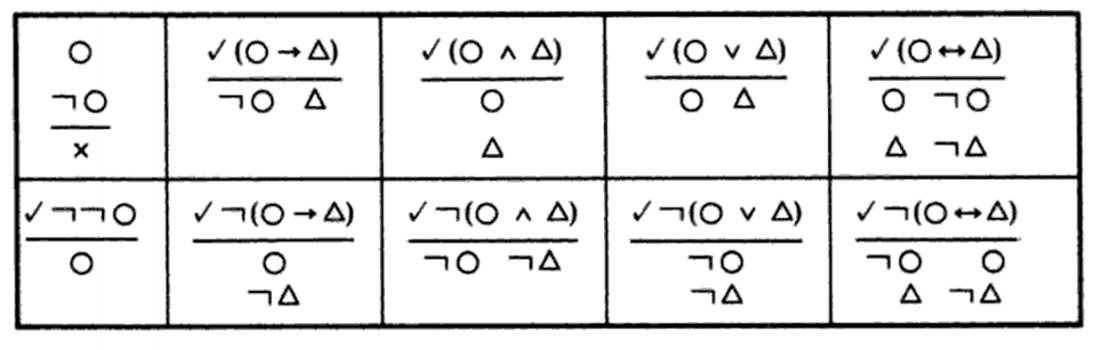
\includegraphics[height=2.6cm]{rules.png}\par
  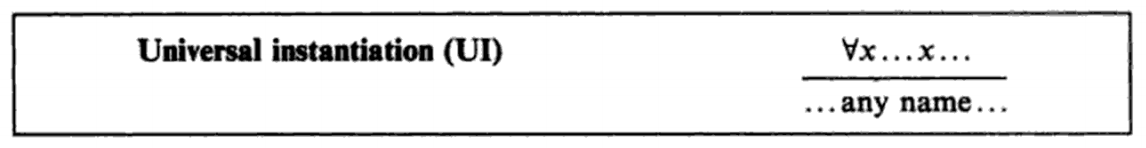
\includegraphics[height=1cm]{ui.png}\par
  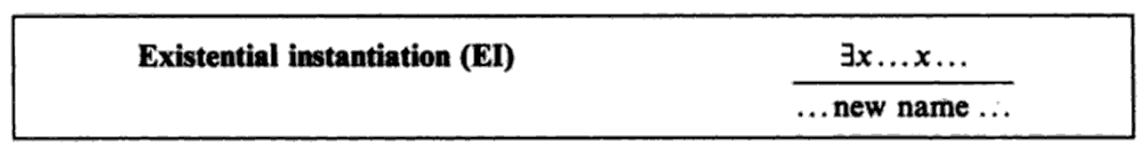
\includegraphics[height=1cm]{ei.png}\par
\end{multicols}
\begin{center}
  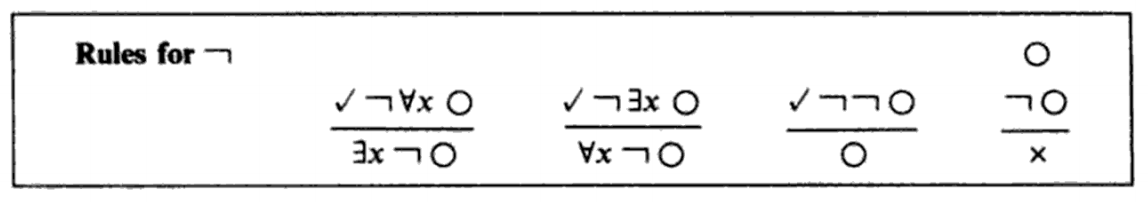
\includegraphics[height=2cm]{not_ui_ei.png}
\end{center}

\section*{Rules of Formation}
\begin{enumerate}[start=0]
  \item $P_a$, $R_{cd}$, $A$, or $B$ where ${a,b,c,d...}$ are names and ${P,R,A,B,...}$ are predicates.
  \item If $\s$ is a sentence, so is $\neg\s$.
  \item If $\s$ and $\t$ are sentences, so are $(\s \land \t)$, $(\s \lor \t)$, $(\s \leftrightarrow \t)$, $(\s \rightarrow \t)$
  \item If $...n...$ is a sentence, so are $\exists x ... x ...$ and $\forall x ... x ...$  
\end{enumerate}

\section*{Truth Tables}
\begin{tabular}{cc|cccc}
  $A$ & $B$ & $A \land B$ & $A \lor B$ & $A \rightarrow C$ & $B \leftrightarrow C$ \\ \hline
  t & t & t & t & t & t \\
  t & f & f & t & f & f \\
  f & t & f & t & t & f \\
  f & f & f & f & t & t
\end{tabular}
\\ \\
$A \rightarrow B$ is logically equivalent to $\neg A \lor B$ \\
$A \leftrightarrow B$ is logically equivalent to $(A \rightarrow B) \land (B \rightarrow A)$

\section*{Validity and Consistency}
\subsubsection*{\underline{Using Truth Tables}}
\textbf{Argument Validity:} An  argument  is  valid  if  and  only  if  the  premises  and  the  negation  of  the conclusion are inconsistent.

\subsubsection*{\underline{Using Refutation Trees}}
\textbf{Argument Validity:} If the refutation tree is inconsistent, the argument is valid. \\
\textbf{Consistency:} A set of sentences is consistent if the sentences can all be true at the same time.  The set is inconsistent if the sentences are never all true at the same time. When all paths of a refutation tree close, the sentences are inconsistent. If there are paths open, they are consistent. \\
\textbf{Tautology:} Create a refutation tree for an argument (negate it), if the tree closes, it is a tautology.
\textbf{Sentence Equivalence:} For sentences $A$ and $B$, you can check if they are consistent by forming a refutation tree for $\neg(A \leftrightarrow B)$ and see if all paths close.
\begin{multicols}{2}
  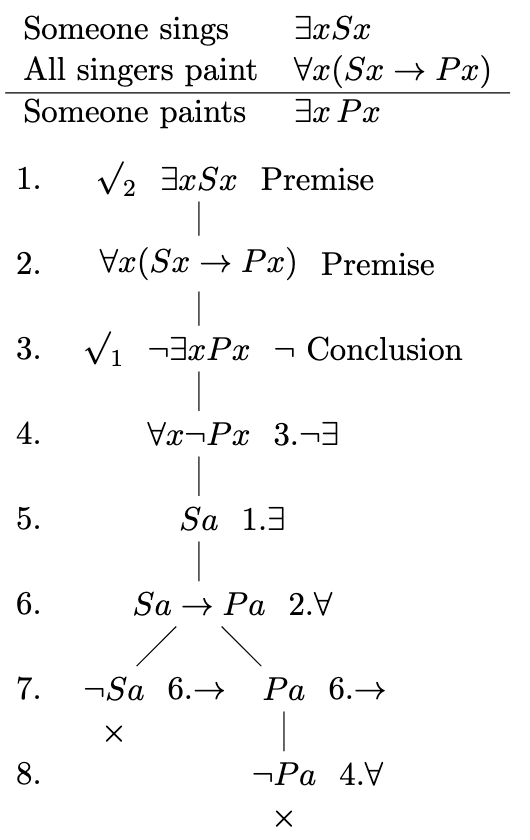
\includegraphics[width=6cm]{reftree.png}\par
  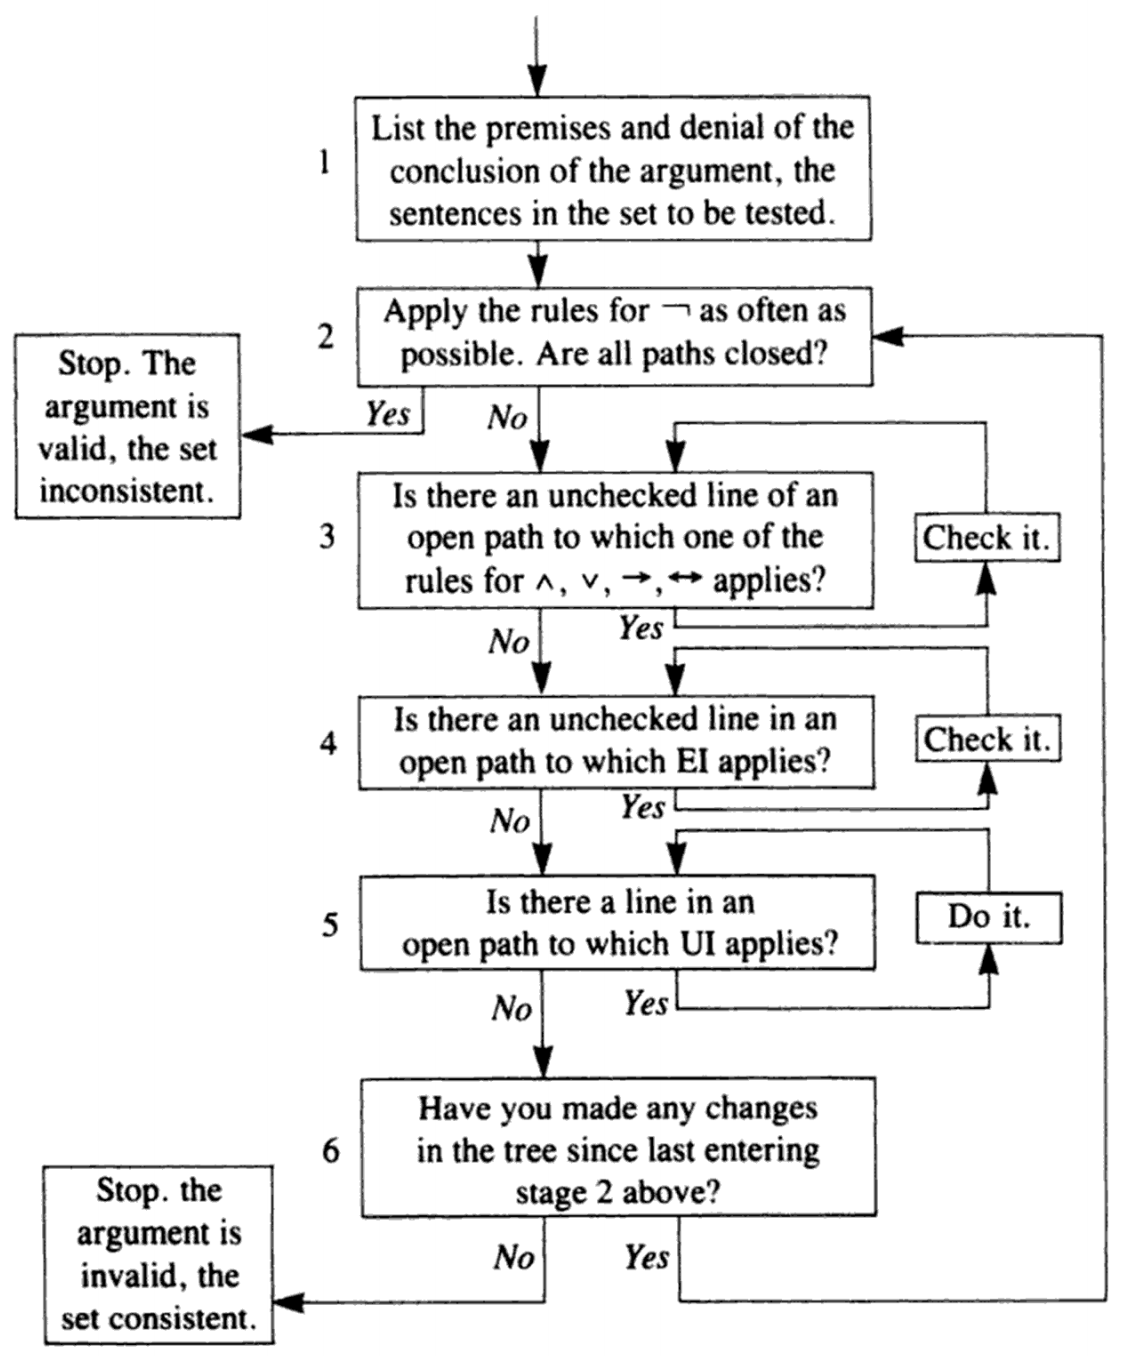
\includegraphics[width=8cm]{flow.png}\par
\end{multicols}


\end{document}

